%%%%%%%%%%%%%%%%%%%%%%%%%%%%%%%%%%%%%%%%%%%%%%%%%%%%%%%%%%%%%%%%%%%%%%%%%%%%%%%%%%%%%%%%%%%%%%%%%
%
% Document:     DM Support Prd.  product tree
%
%%%%%%%%%%%%%%%%%%%%%%%%%%%%%%%%%%%%%%%%%%%%%%%%%%%%%%%%%%%%%%%%%%%%%%%%%%%%%%
\documentclass{article}
\usepackage{times,layouts}
\usepackage{tikz,hyperref,amsmath}
\usetikzlibrary{positioning,arrows,shapes,decorations.shapes,shapes.arrows}
\usetikzlibrary{backgrounds,calc}
\usepackage[paperwidth=1015.9999999999998pt,paperheight=559pt,
left=-2mm,top=3mm,bottom=0mm,right=0mm,
noheadfoot,marginparwidth=0pt,includemp=false,
textwidth=30cm,textheight=50mm]{geometry}
\newcommand\showpage{%
\setlayoutscale{0.5}\setlabelfont{\tiny}\printheadingsfalse\printparametersfalse
\currentpage\pagedesign}
\hypersetup{pdftitle={DM Support Prd. products }, pdfsubject={Diagram illustrating the
                products in LSST DM Support Prd. }, pdfauthor={Extracted from MagicDraw}}
\tikzstyle{tbox}=[rectangle,text centered, text width=30mm]
\tikzstyle{wbbox}=[rectangle, rounded corners=3pt, draw=black, top color=blue!50!white,
                    bottom color=white, very thick, minimum height=40pt, inner sep=2pt,
                    text centered, text width=30mm]
\tikzstyle{pbox}=[rectangle, rounded corners=3pt, draw=black, top
 color=yellow!50!white, bottom color=white, very thick,
 minimum height=36pt, inner sep=3pt, text centered, text width=35mm]
\tikzstyle{pline}=[-, thick]
\begin{document}
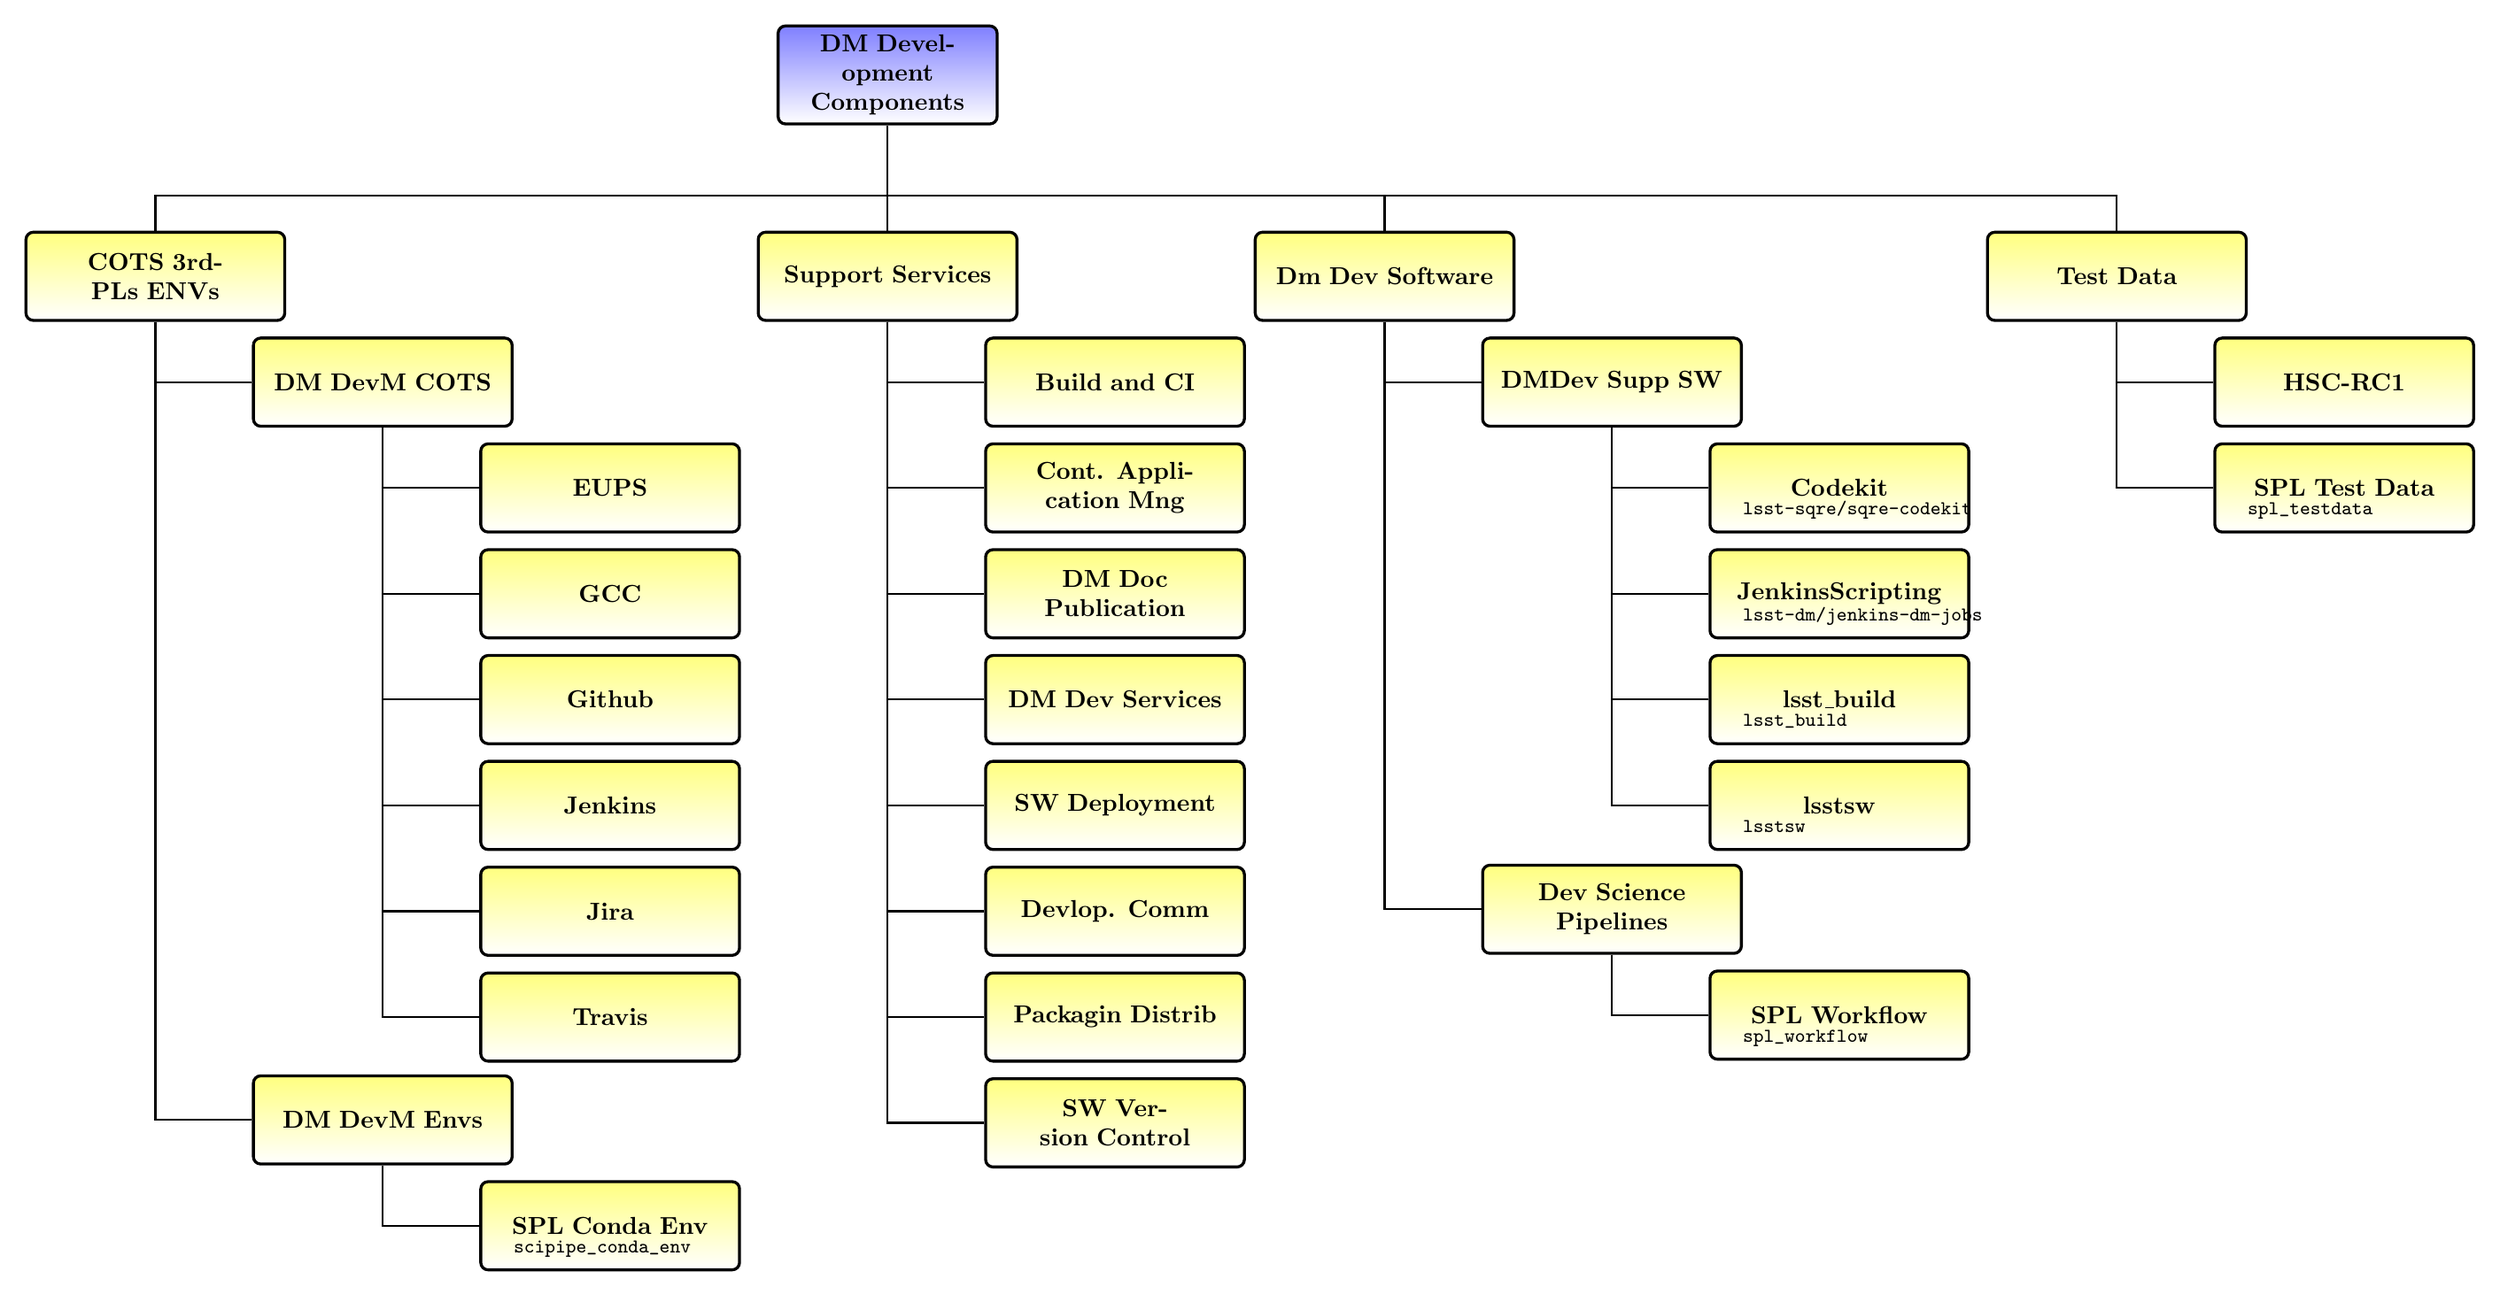
\begin{tikzpicture}[node distance=0mm]


\node (DMDC3E) [pbox, 
] {\textbf{COTS 3rdPLs ENVs
} };\node [below right] at (DMDC3E.north west) {\footnotesize \color{blue}} ;

\node (COTSDM) [pbox,below right=6pt and -14pt of DMDC3E] {\textbf{DM DevM COTS
} };\node [below right] at (COTSDM.north west) {\footnotesize \color{blue}} ;

 \draw[pline] (DMDC3E.south) -| ++(0,0) |- (COTSDM.west); 
\node (EUPS) [pbox,below right=6pt and -14pt of COTSDM] {\textbf{EUPS
} };\node [below right] at (EUPS.north west) {\footnotesize \color{blue}} ;

 \draw[pline] (COTSDM.south) -| ++(0,0) |- (EUPS.west); 
\node (GCC) [pbox,below=6pt of EUPS] {\textbf{GCC
} };\node [below right] at (GCC.north west) {\footnotesize \color{blue}} ;

 \draw[pline] (COTSDM.south) -| ++(0,0) |- (GCC.west); 
\node (GITHUB) [pbox,below=6pt of GCC] {\textbf{Github
} };\node [below right] at (GITHUB.north west) {\footnotesize \color{blue}} ;

 \draw[pline] (COTSDM.south) -| ++(0,0) |- (GITHUB.west); 
\node (JNKNS) [pbox,below=6pt of GITHUB] {\textbf{Jenkins
} };\node [below right] at (JNKNS.north west) {\footnotesize \color{blue}} ;

 \draw[pline] (COTSDM.south) -| ++(0,0) |- (JNKNS.west); 
\node (JRA) [pbox,below=6pt of JNKNS] {\textbf{Jira
} };\node [below right] at (JRA.north west) {\footnotesize \color{blue}} ;

 \draw[pline] (COTSDM.south) -| ++(0,0) |- (JRA.west); 
\node (TRVS) [pbox,below=6pt of JRA] {\textbf{Travis
} };\node [below right] at (TRVS.north west) {\footnotesize \color{blue}} ;

 \draw[pline] (COTSDM.south) -| ++(0,0) |- (TRVS.west); 
\node (DENV) [pbox,below=264pt of COTSDM] {\textbf{DM DevM Envs
} };\node [below right] at (DENV.north west) {\footnotesize \color{blue}} ;

 \draw[pline] (DMDC3E.south) -| ++(0,0) |- (DENV.west); 
\node (SPLCE) [pbox,below right=6pt and -14pt of DENV] {\textbf{SPL Conda Env
} };\node [below right] at (SPLCE.north west) {\footnotesize \color{blue}} ;
\node (SPLCEpkg) [tbox,below=3mm of SPLCE.north] {{\footnotesize \color{black} \begin{verbatim} scipipe_conda_env \end{verbatim} }  };

 \draw[pline] (DENV.south) -| ++(0,0) |- (SPLCE.west); 
\node (DMDSRV) [pbox, 
right=192pt of DMDC3E] {\textbf{Support Services
} };\node [below right] at (DMDSRV.north west) {\footnotesize \color{blue}} ;

\node (BCI) [pbox,below right=6pt and -14pt of DMDSRV] {\textbf{Build and CI
} };\node [below right] at (BCI.north west) {\footnotesize \color{blue}} ;

 \draw[pline] (DMDSRV.south) -| ++(0,0) |- (BCI.west); 
\node (CAM) [pbox,below=6pt of BCI] {\textbf{Cont. Application Mng
} };\node [below right] at (CAM.north west) {\footnotesize \color{blue}} ;

 \draw[pline] (DMDSRV.south) -| ++(0,0) |- (CAM.west); 
\node (DDCPUB) [pbox,below=6pt of CAM] {\textbf{DM Doc Publication
} };\node [below right] at (DDCPUB.north west) {\footnotesize \color{blue}} ;

 \draw[pline] (DMDSRV.south) -| ++(0,0) |- (DDCPUB.west); 
\node (DDVSRV) [pbox,below=6pt of DDCPUB] {\textbf{DM Dev Services
} };\node [below right] at (DDVSRV.north west) {\footnotesize \color{blue}} ;

 \draw[pline] (DMDSRV.south) -| ++(0,0) |- (DDVSRV.west); 
\node (DEPLOY) [pbox,below=6pt of DDVSRV] {\textbf{SW Deployment
} };\node [below right] at (DEPLOY.north west) {\footnotesize \color{blue}} ;

 \draw[pline] (DMDSRV.south) -| ++(0,0) |- (DEPLOY.west); 
\node (DMDCOM) [pbox,below=6pt of DEPLOY] {\textbf{Devlop. Comm
} };\node [below right] at (DMDCOM.north west) {\footnotesize \color{blue}} ;

 \draw[pline] (DMDSRV.south) -| ++(0,0) |- (DMDCOM.west); 
\node (PKGDST) [pbox,below=6pt of DMDCOM] {\textbf{Packagin Distrib
} };\node [below right] at (PKGDST.north west) {\footnotesize \color{blue}} ;

 \draw[pline] (DMDSRV.south) -| ++(0,0) |- (PKGDST.west); 
\node (SWVER) [pbox,below=6pt of PKGDST] {\textbf{SW Version Control
} };\node [below right] at (SWVER.north west) {\footnotesize \color{blue}} ;

 \draw[pline] (DMDSRV.south) -| ++(0,0) |- (SWVER.west); 
\node (DMDSW) [pbox, 
right=96pt of DMDSRV] {\textbf{Dm Dev Software
} };\node [below right] at (DMDSW.north west) {\footnotesize \color{blue}} ;

\node (DMDSS) [pbox,below right=6pt and -14pt of DMDSW] {\textbf{DMDev Supp SW
} };\node [below right] at (DMDSS.north west) {\footnotesize \color{blue}} ;

 \draw[pline] (DMDSW.south) -| ++(0,0) |- (DMDSS.west); 
\node (CDKT) [pbox,below right=6pt and -14pt of DMDSS] {\textbf{Codekit
} };\node [below right] at (CDKT.north west) {\footnotesize \color{blue}} ;
\node (CDKTpkg) [tbox,below=3mm of CDKT.north] {{\footnotesize \color{black} \begin{verbatim} lsst-sqre/sqre-codekit \end{verbatim} }  };

 \draw[pline] (DMDSS.south) -| ++(0,0) |- (CDKT.west); 
\node (JSCR) [pbox,below=6pt of CDKT] {\textbf{JenkinsScripting
} };\node [below right] at (JSCR.north west) {\footnotesize \color{blue}} ;
\node (JSCRpkg) [tbox,below=3mm of JSCR.north] {{\footnotesize \color{black} \begin{verbatim} lsst-dm/jenkins-dm-jobs \end{verbatim} }  };

 \draw[pline] (DMDSS.south) -| ++(0,0) |- (JSCR.west); 
\node (LBLD) [pbox,below=6pt of JSCR] {\textbf{lsst\_build
} };\node [below right] at (LBLD.north west) {\footnotesize \color{blue}} ;
\node (LBLDpkg) [tbox,below=3mm of LBLD.north] {{\footnotesize \color{black} \begin{verbatim} lsst_build \end{verbatim} }  };

 \draw[pline] (DMDSS.south) -| ++(0,0) |- (LBLD.west); 
\node (LSSTSW) [pbox,below=6pt of LBLD] {\textbf{lsstsw
} };\node [below right] at (LSSTSW.north west) {\footnotesize \color{blue}} ;
\node (LSSTSWpkg) [tbox,below=3mm of LSSTSW.north] {{\footnotesize \color{black} \begin{verbatim} lsstsw \end{verbatim} }  };

 \draw[pline] (DMDSS.south) -| ++(0,0) |- (LSSTSW.west); 
\node (DSPLSW) [pbox,below=178pt of DMDSS] {\textbf{Dev Science Pipelines
} };\node [below right] at (DSPLSW.north west) {\footnotesize \color{blue}} ;

 \draw[pline] (DMDSW.south) -| ++(0,0) |- (DSPLSW.west); 
\node (SPLWF) [pbox,below right=6pt and -14pt of DSPLSW] {\textbf{SPL Workflow
} };\node [below right] at (SPLWF.north west) {\footnotesize \color{blue}} ;
\node (SPLWFpkg) [tbox,below=3mm of SPLWF.north] {{\footnotesize \color{black} \begin{verbatim} spl_workflow \end{verbatim} }  };

 \draw[pline] (DSPLSW.south) -| ++(0,0) |- (SPLWF.west); 
\node (DMDTDP) [pbox, 
right=192pt of DMDSW] {\textbf{Test Data
} };\node [below right] at (DMDTDP.north west) {\footnotesize \color{blue}} ;

\node (HSCRC1) [pbox,below right=6pt and -14pt of DMDTDP] {\textbf{HSC-RC1
} };\node [below right] at (HSCRC1.north west) {\footnotesize \color{blue}} ;

 \draw[pline] (DMDTDP.south) -| ++(0,0) |- (HSCRC1.west); 
\node (SPLTD) [pbox,below=6pt of HSCRC1] {\textbf{SPL Test Data
} };\node [below right] at (SPLTD.north west) {\footnotesize \color{blue}} ;
\node (SPLTDpkg) [tbox,below=3mm of SPLTD.north] {{\footnotesize \color{black} \begin{verbatim} spl_testdata \end{verbatim} }  };

 \draw[pline] (DMDTDP.south) -| ++(0,0) |- (SPLTD.west); 
\node (DMDEV) [wbbox, above=43pt of DMDSRV]{\textbf{DM Development Components}};
 \draw[pline]   (DMDC3E.north) -- ++(0.0,0.5) -| (DMDEV.south) ; 
 \draw[pline]   (DMDSRV.north) -- ++(0.0,0.5) -| (DMDEV.south) ; 
 \draw[pline]   (DMDSW.north) -- ++(0.0,0.5) -| (DMDEV.south) ; 
 \draw[pline]   (DMDTDP.north) -- ++(0.0,0.5) -| (DMDEV.south) ; 

\end{tikzpicture}
\end{document}
